\documentclass{book}
\setlength{\evensidemargin}{0in}
\setlength{\oddsidemargin}{0in}
\setlength{\textwidth}{7.0in}
\setlength{\parskip}{10pt}
\setlength{\parindent}{0in}
\usepackage{graphicx}
\usepackage{amsmath}
\usepackage{underscore}
\usepackage{float}
%\usepackage{mathptmx}
\usepackage{fix-cm}
%\usepackage{relsize}
%\usepackage{floatrow}
\usepackage{rotate}
\usepackage[singlelinecheck=off]{caption}
%\usepackage{caption}
\usepackage{subcaption}
%\usepackage[left=2cm,top=1cm,right=3cm,nohead,nofoot]{geometry}
\usepackage[left=2cm,top=2cm,right=2cm]{geometry}

%%%%%%%%%%%%%%%%%%%%%%%%%%%%%%%%%%%%%%%%%%%%%%%%%%%%%%%
%\voffset = 20pt
\begin{document}

%%%%%%%%%%%%%%%%%%%%%%%%%%%%%%%%%%%%%%%%%%%%%%%%%%%%%%%

%%%start

\section{Vacuum Technology Laboratory}

{\bf Note: This lab is designed to be done in Science Theaters 029}\newline

%%%%%%%%%%%%%%%%%%%%%%%%%%%%%%%%%%%%%%%%%%%%%%%%%%%%%%%%%%%%%%
%Setup
%%%%%%%%%%%%%%%%%%%%%%%%%%%%%%%%%%%%%%%%%%%%%%%%%%%%%%%%%%%%%%

\subsection{Experimental Setup}

{\bf Equipmnent List:}

I)    Hand operated vacuum pump, Edwards RV5 mechanical pump, schematic diagram of vacuum pumping principles, 5 board-mounted gauges.\newline
II)   Sorption pump, liquid nitrogen and dewar, thermocouple vacuum gauge, safety glasses, heat gun.\newline
III)  "Leaky weld" assembly, Edwards RV5 mechanical pump, helium bottle with regulator and bench clamp, 2 labs stands, 2 fork clamps, 2 right-angle clamps.\newline
IV)   Vacuum manifold cart, Edwards RV5 mechanical pump, 2 anatek power supplies, connecting leads.\newline
V)    Edwards RV5 mechanical pump, foreline trap, 2 isolation valves, vacuum hose, 25cm tube with NW25 terminations, four-way cross with NW25 flanges, thermocouple vacuum guage, assortment of NW25 O-rings and metal centering rings. assortment of NW25 clamps, rubber gloves.\newline
VI)   Vernier capable computer, Vernier intrumentation amplifier, pumpdown_template.cmbl Loggerpro file, pumpdown and leakout curve apparatus, stopwatch.\newline
VII)  Diffstak equipment cart, RG-83 ionization guage controller, Edwards RV5 mechanical vacuum pump.
VIII) High Vacuum Turbo Molecular System.\newline
Components of vacuum system museum that match labels available in "label" section.\newline

%%%%%%%%%%%%%%%%%%%%%%%%%%%%%%%%%%%%%%%%%%%%%%%%%%%%%%%%%%%%%%
%Room Layout
%%%%%%%%%%%%%%%%%%%%%%%%%%%%%%%%%%%%%%%%%%%%%%%%%%%%%%%%%%%%%%

\subsection{Room Layout}

\begin{figure}[H]
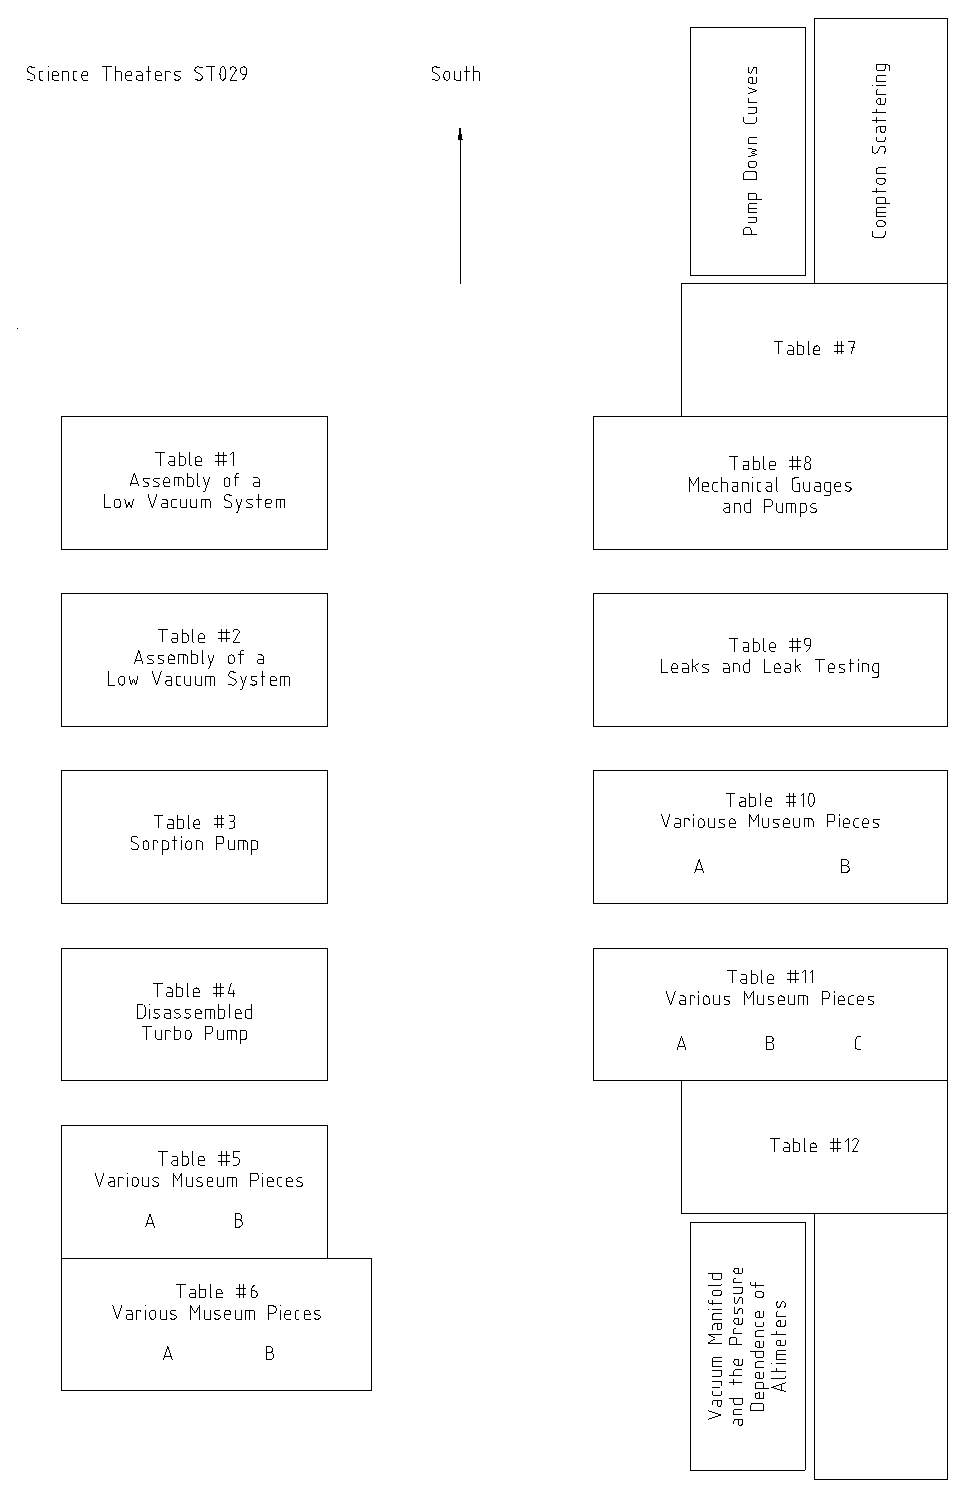
\includegraphics[scale=1.0]{room-layout.eps}
\caption{Layout of Room}
\label{Layout of Room}
\end{figure}

\subsection{Table Layout}

\subsubsection{Table 1: Assembly of a Low Vacuum System}

\begin{figure}[H]
\centering
\begin{subfigure}{.5\textwidth} 
  \centering
  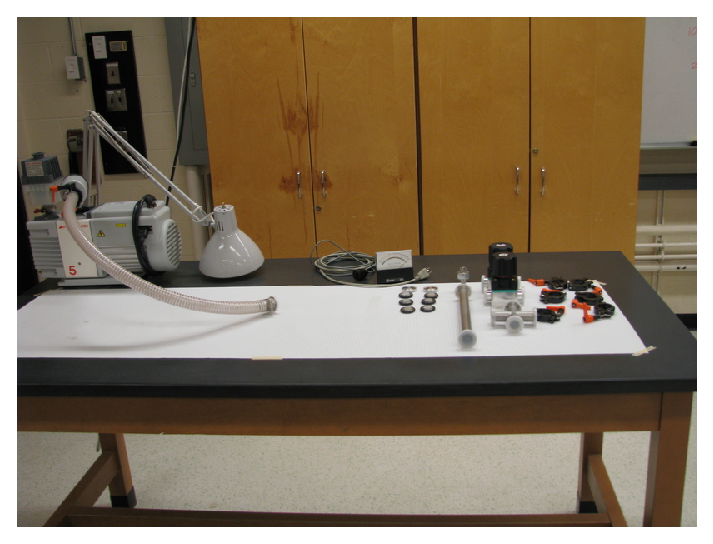
\includegraphics[width=0.95\linewidth]{Low-Vacuum-System-Table1-2}
  \caption{Equimpent arranged for the student} 
  \label{For Storage - Assembly of a Low Vacuum System}
\end{subfigure}%
\begin{subfigure}{.5\textwidth}
  \centering
  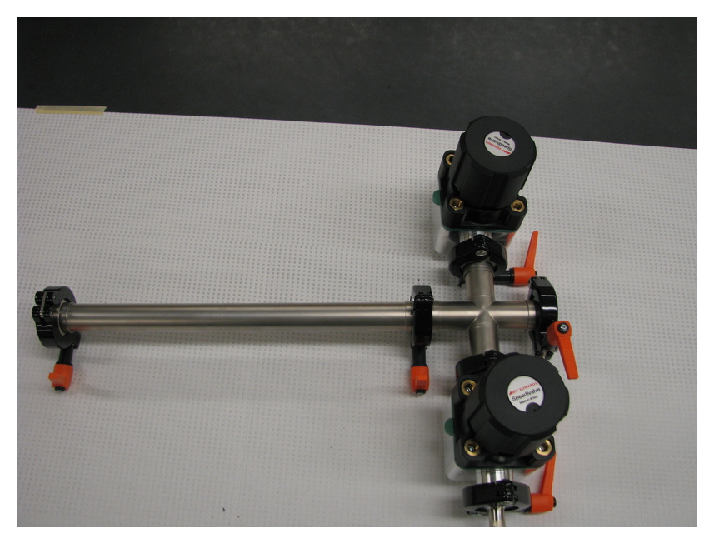
\includegraphics[width=0.95\linewidth]{Low-Vacuum-System-Assembled-Table1-2}
  \caption{Equipment assembled for storage}
  \label{For Student - Assembly of a Low Vacuum System} 
\end{subfigure}
\caption{Table 1 Contians: Edwards RV5 pump, foreline trap, 2 isolation valves, vacuum hose, 25 cm tube with NW25 terminations, four-way cross with NW25 flanges, Varian vacuum gauge and gauge head, assorment of NW25 rubber O-rings and metal centering rings, assortment of NW25 clamps, and rubber gloves.}
\label{fig:test}
\end{figure}

\subsubsection{Table 2: Assembly of a Low Vacuum System}
Table 2 should be identical to Table 1

\subsubsection{Table 3: Pumping with No Moving Parts}

\begin{figure}[H]
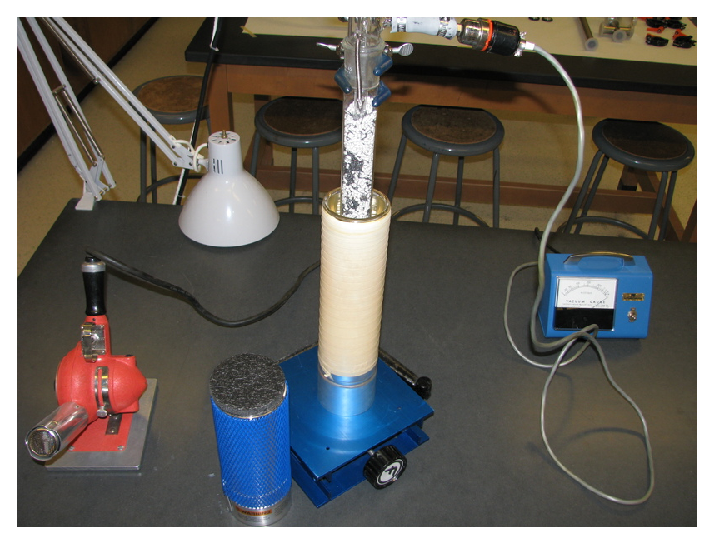
\includegraphics[scale=0.8]{Sorption-Pump-Table3}
\caption[align=left]{Table8 3 Contains: sorption pump, lab jack, tc gauge and guage head, tall liquid nitrogen dewer, second liquid nitrogen dewer, heat gun, and safety glasses (not shown).}
\end{figure}

\subsubsection{Table 4: Dissasembled Turbo Pump}

\begin{figure}[H]
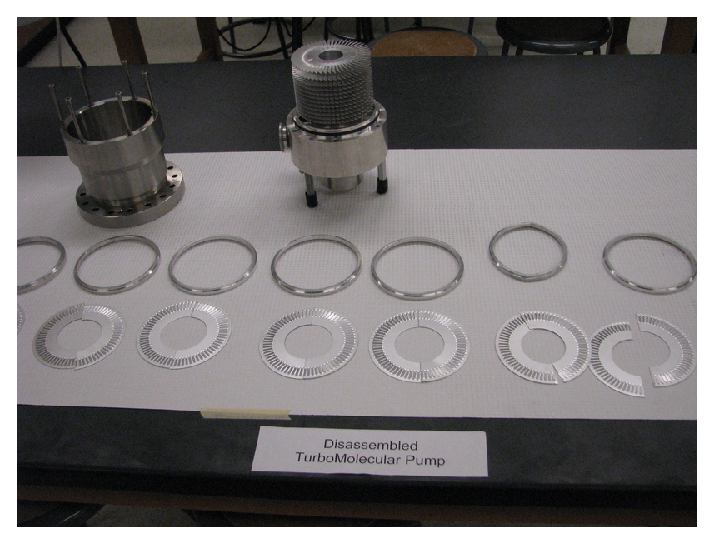
\includegraphics[scale=0.8]{Turbo-Pump-Table4}
\caption[align=left]{Table 4 Contains: dissasembled turbo pump.}
\end{figure}

\subsubsection{Table 5: Various Museum Pieces}

\begin{figure}[H]
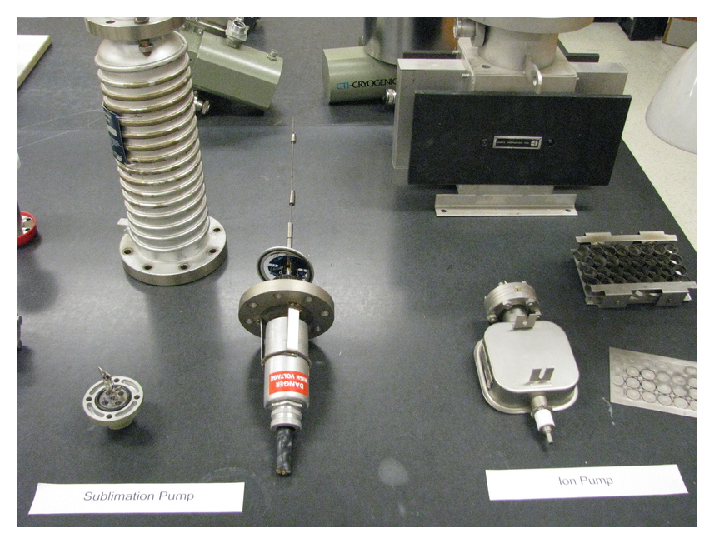
\includegraphics[scale=0.9]{Museum-Pieces-Table5A}
\caption[align=left]{Table 5A Contains: sublimation pump and ion pump.}
\end{figure}


\begin{figure}[H]
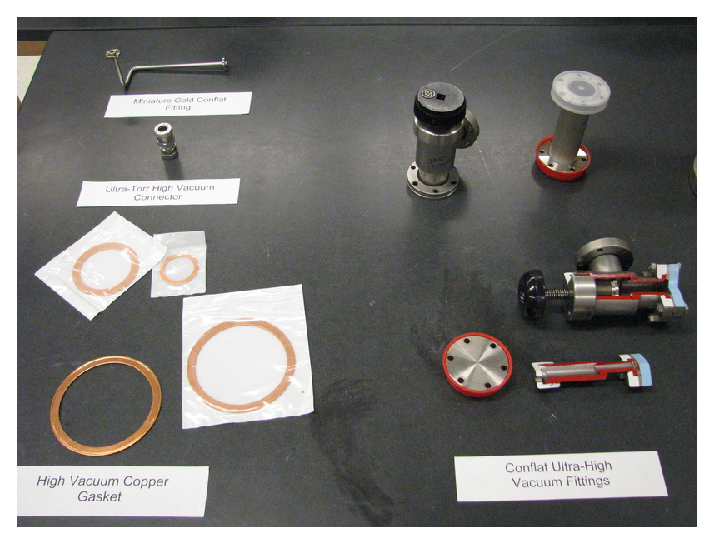
\includegraphics[scale=0.9]{Museum-Pieces-Table5B}
\caption{Tabel 5B Contains: miniature gold conflat fitting, ultra-torr high vacuum connector, high vacuum copper gasket, and conflat ultra-high vacuum fittings.}
\end{figure}

\subsubsection{Table 6: Various Museum Pieces}

\begin{figure}[H]
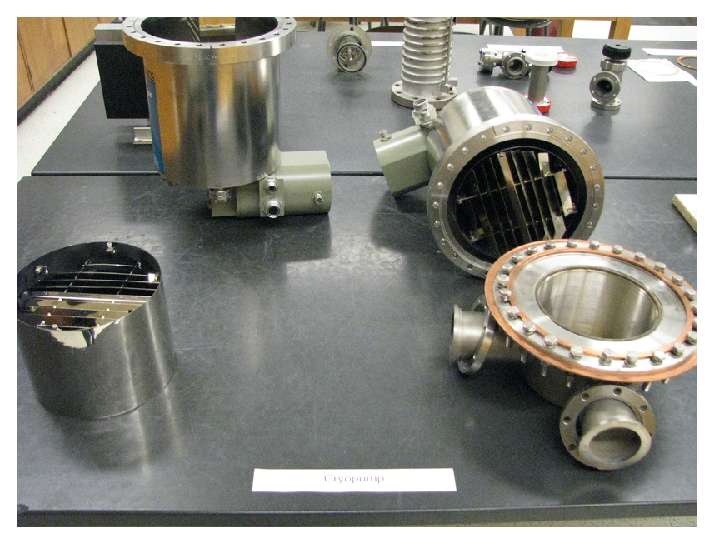
\includegraphics[scale=0.9]{Museum-Pieces-Table6A}
\caption[align=left]{Table 6A Contains: cryopump.}
\end{figure}

\begin{figure}[H]
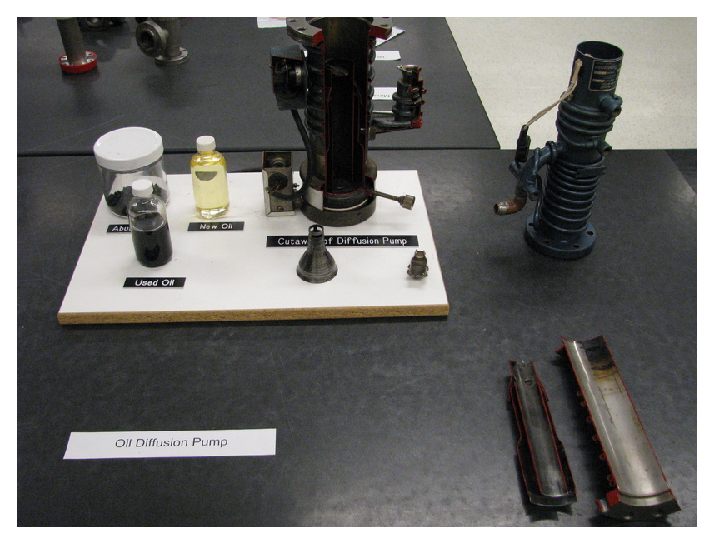
\includegraphics[scale=0.9]{Museum-Pieces-Table6B}
\caption[align=left]{Table 6A Contains: oil diffusion pump.}
\end{figure}

\subsubsection{Table 7: Empty }
Table 7 should remain empty

\subsubsection{Table 8: Mechanical Gauges and Pumps}

\begin{figure}[H]
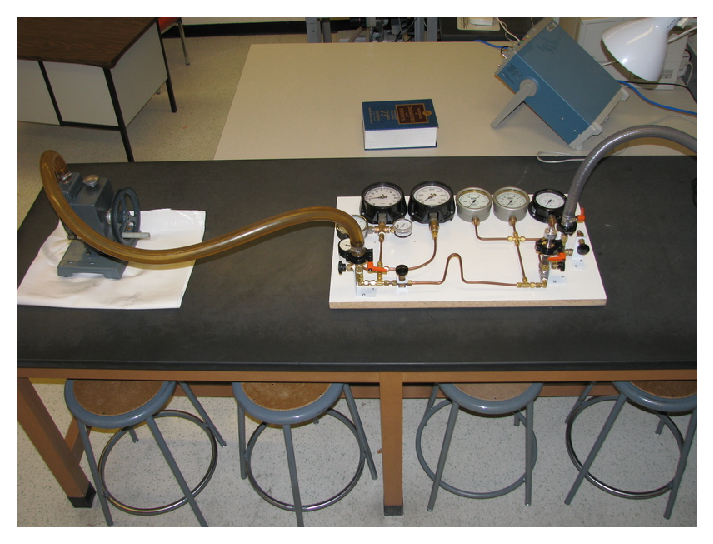
\includegraphics[scale=0.9]{Mechanical-Gauges-and-Pumps-Table8}
\caption[align=left]{Table 8 Contains: hand operated vacuum pump. Edwards RV5 mechanical pump, schematic diagram of vacuum pumping principles, and 5 board-mounted gauges.}
\end{figure}

\subsubsection{Table 9: Leaks and Leak Testing}

\begin{figure}[H]
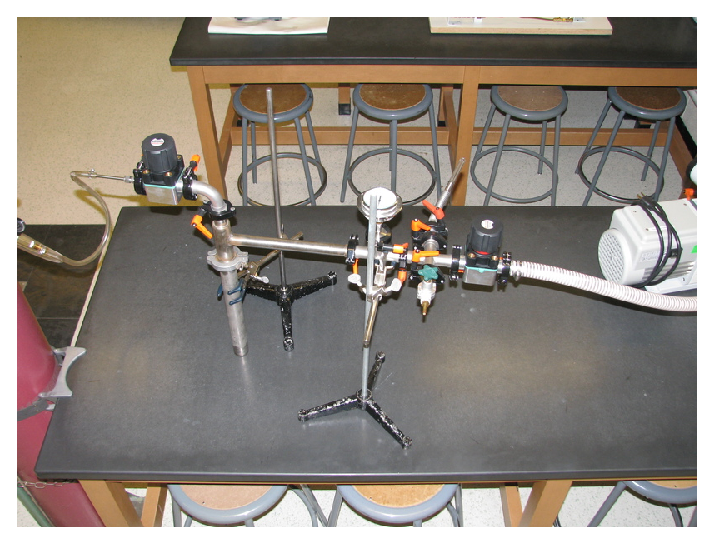
\includegraphics[scale=0.9]{Leaks-and-Leak-Testing-Table9}
\caption[align=left]{Table 9 Contains: "Leaky Weld" assembly, Edwards RV5 mechanical pump, helium bottle with regulator and bench clamp, 2 lab standss, 2 fork clamps, and 2 right-angle clamps.}
\end{figure}

\subsubsection{Table 10: Various Museam Pieces}

\begin{figure}[H]
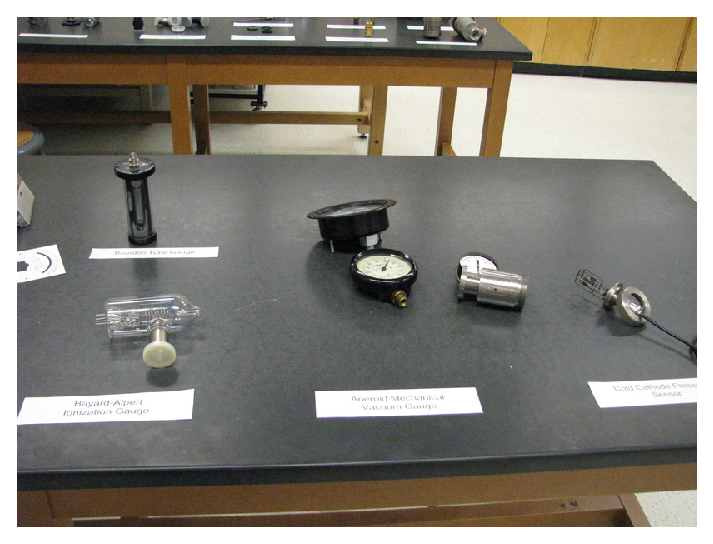
\includegraphics[scale=0.9]{Museum-Pieces-Table10A}
\caption[align=left]{Table 10A Contains: Bourdon tube gauge, Bayard-Alpert ionization gauge, Aneroid mechanical vacuum gauge, cold cathode pressure sensor.}
\end{figure}

\begin{figure}[H]
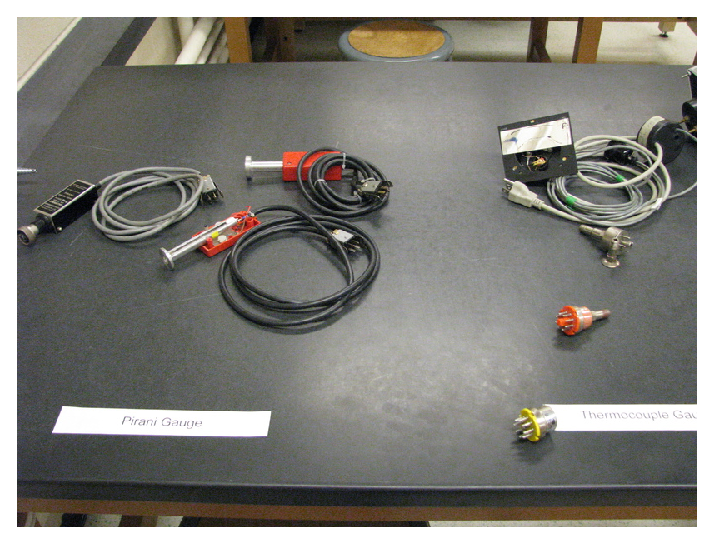
\includegraphics[scale=0.9]{Museum-Pieces-Table10B}
\caption[align=left]{Table 10B Contains: Pirani gauge and thermocouple gauge.}
\end{figure}

\subsubsection{Table 11: Various Museam Pieces}

\begin{figure}[H]
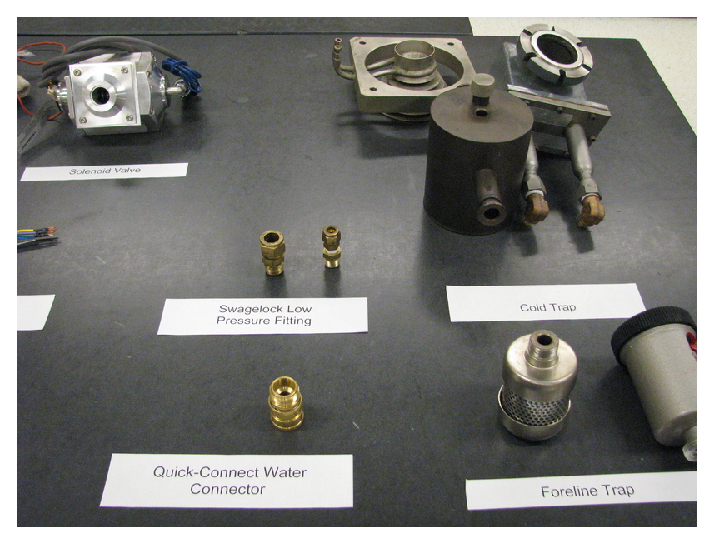
\includegraphics[scale=0.9]{Museum-Pieces-Table11A}
\caption[align=left]{Table 11A Contains: swagelock low pressure fitting, cold trap, quick-connect water connector, and foreline trap.}
\end{figure}

\begin{figure}[H]
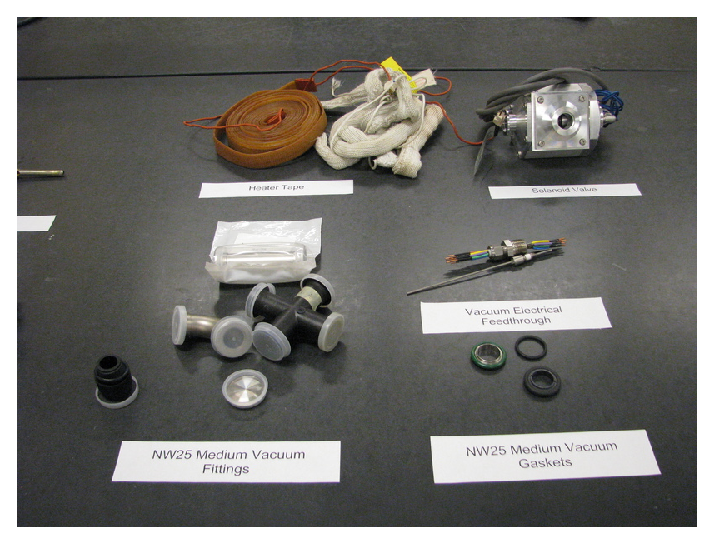
\includegraphics[scale=0.9]{Museum-Pieces-Table11B}
\caption[align=left]{Table 11B Contains: heater tape, solenoid valve, NW25 medium vacuum fittings, NW25 medium Vacuum Gaskets, and vacuum electrical feedthrough.}
\end{figure}

\begin{figure}[H]
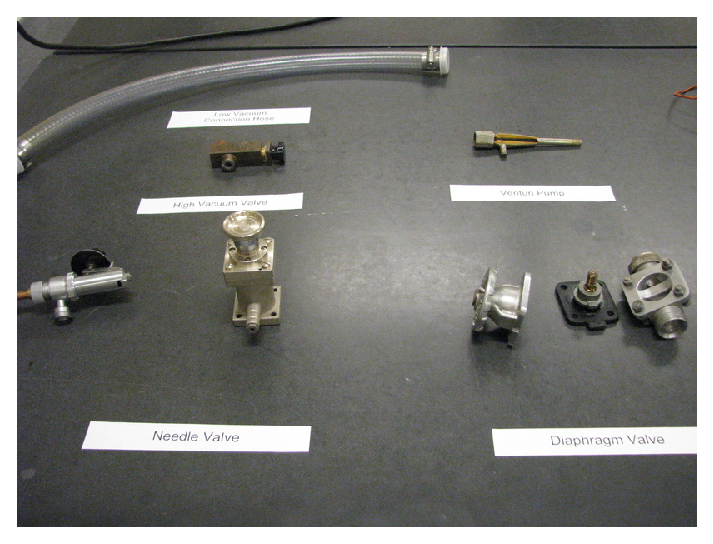
\includegraphics[scale=0.9]{Museum-Pieces-Table11C}
\caption[align=left]{Table 11C Contains: low vacuum cnnection hose, high vacuum valve, venturi pump, needle valve, and diaphragm valve.}
\end{figure}

\subsubsection{Pump Down Curves}

\begin{figure}[H]
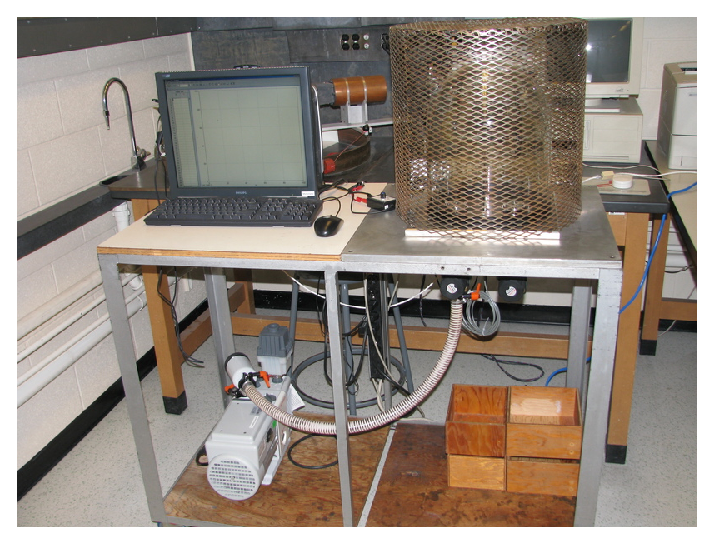
\includegraphics[scale=0.9]{Pump-Down-Curves}
\caption[align=left]{Contains: Vernier capable computer, Vernier instrument amplifier, pumpdown_template.cmbl file, pumpdown and leakout curve apparatus, and stopwatch}
\end{figure}

\subsubsection{Vacuum Manifold and the Pressure Dependance of Altimeters}

\begin{figure}[H]
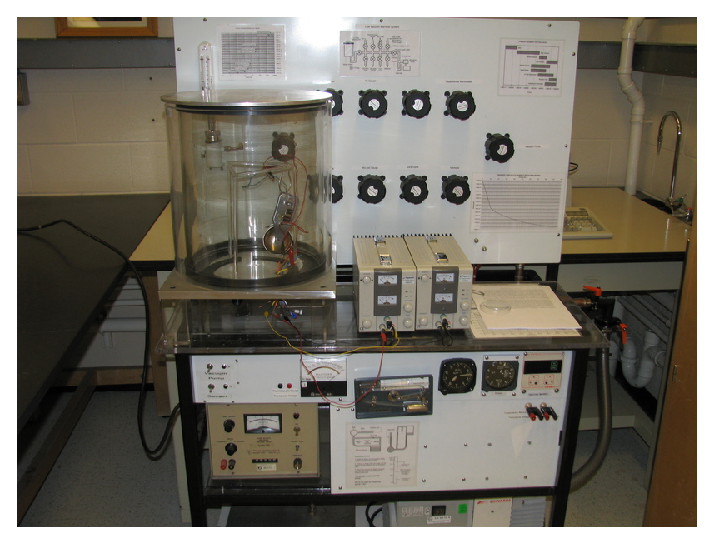
\includegraphics[scale=0.9]{Manifold-System}
\caption[align=left]{Contains: vacuum manifold cart, Edwards RV5 pump, 2DC power supplies, connecting leads.}
\end{figure}

\newpage

{\subsection{Notes to the Instructor}
{\bf Equipmnent Care:}

Startup procedure for diffstak vacuum system.\newline
A) Turn on water for cooling system\newline
B) Close vent valve, main chamber valve, chamber backing valve, and backing valve.\newline
C) Turn on mechanical pump, and guage controller.\newline
D) Open backing valve and chamber backing valve, and pump on system until pressure in main chamber, and backing pipe have a pressure of less then 10mTorr.\newline
E) Turn on diffusion pumb, and allow the oil to warm up for 10 minutes.\newline
F) Open main chamber valve. If the backing pressure raises above 50mTorr close the main chamber valve and allow the mechanical pump or pump on the system for another 30 minutes. Continue this until the backing pressure remains below 50mTorr.\newline
G) Turn on ion Guage.\newline

Shutdown procedure for diffstak vacuum system.\newline
A) Close main chamber valve, and turn off diffusion pump.\newline 
B) Allow water to run for 30 minutes.\newline
C) Turn off water, mechanical pumb, and guages. Do not open vent valve.\newline

Startup procedure for the Turbo Molecular Pump.\newline
A) Turn on water for cooling system.\newline
B) Turn on guages, and mechanical pump.\newline
C) Pump on the backing side of the system until the backing pressure is less then 5mTorr.\newline
D) Open the main chamber up to the mechanical pump and allow it to pump down on the whole system until the chamber is less then 5mTorre.\newline
E) Turn on the turbo pump with high frequency and pump down on the whole system.\newline
F) Turn on the ion gauge and keep an eye on the progress. The system should eventually bottom out the ion guage.\newline
G) Once the pressure is in 10e-7 the ion pump can be turned on to help with pump down.\newline
H) Once the load on the ion pump is low turn the frequency of the turbo pump to low.\newline

Shutdown procedure for the Turbo Molecular Pump.\newline
A) Close the main chamber valve. \newline
B) Turn off ion pump and turbo molecular pump.\newline
C) Alow system to cool for 30 minutes.\newline
D) Turn of water, mechanical pump, and guages.\newline

{\bf Common Errors made by Students:}
No notes on common errors made by students

{\bf Sample Data:}
No sample data.

\subsection{Maintenance}

A) If a pump has not been used for awhile it may need to be seasoned. An unseasoned pump can appear as a leak in the system. The pump may need to be ran for up to a week in order remove excess water and other contaminants from the system. \newline
B) Check the colour and level of the oil in the mechanical pumps before each use.\newline
C) Check vacuum log for further instruction on when to change the oil of the diffstack and turbo pumps.\newline

\newpage
\subsection{Labels}
\begin{centering}
\fontsize{48}{48}\selectfont
Bourdon Tube Gauge\\
\vspace{30 mm}
Sublimation Pump\\
\vspace{30 mm}
Ion Pump\\
\vspace{30 mm}
Cryopump\\
\vspace{30 mm}
Oil Diffusion Pump\\
\vspace{30 mm}
Solenoid Valve\\
\vspace{30 mm}
Cold Trap\\
\vspace{30 mm}
Foreline Trap\\
\vspace{30 mm}
Heater Tape\\
\vspace{30 mm}
High Vacuum Valve\\
\vspace{30 mm}
Venturi Pump\\
\vspace{30 mm}
Needle Valve\\
\vspace{30 mm}
Diaphragm Valve\\
\vspace{30 mm}
Pirani Gauge\\
\vspace{30 mm}
Thermocouple Gauge\\
\vspace{30 mm}
Bayard-Alpert\\
Ionization Gauge\\
\vspace{30 mm}
Aneroid Mechanical\\
Vacuum Gauge\\
\vspace{30 mm}
Cold Cathode\\ 
Pressure Sensor\\
\vspace{30 mm}
Disassembled\\
TurboMolecular Pump\\
\vspace{30 mm}
Miniature Gold Conflat\\
Fitting\\
\vspace{30 mm}
Ultra-Torr High Vacuum\\
Connector\\
\vspace{30 mm}
High Vacuum\\
Copper Gasket\\
\vspace{30 mm}
Conflat Ultra-High\\
Vacuum Fittings\\
\vspace{30 mm}
Swagelock Low\\
Pressure Fitting\\
\vspace{30 mm}
Quick-Connect\\
Water Connector\\
\vspace{30 mm}
NW25 Medium\\
Vacuum Fittings\\
\vspace{30 mm}
Vacuum Electrical\\
Feedthrough\\
\vspace{30 mm}
NW25 Medium\\
Vacuum Gaskets\\
\vspace{30 mm}
Low Vacuum\\
Connection Hose\\
\vspace{30 mm}
\end{centering}


%%%end

\end{document}

